\documentclass{article}

\usepackage[preprint,nonatbib]{neurips_2026}
\makeatletter
\renewcommand{\@notice}{\enlargethispage{2\baselineskip}}
\makeatother
\raggedbottom

\usepackage[utf8]{inputenc}
\usepackage[T1]{fontenc}
\usepackage{graphicx}
\usepackage{amsmath}
\usepackage{amssymb}
\usepackage{booktabs}
\usepackage{xcolor}
\usepackage{hyperref}
\usepackage{microtype}
\usepackage{caption}
\usepackage{float}
\usepackage[numbers,sort&compress]{natbib}
\renewcommand{\arraystretch}{0.92}
\captionsetup{skip=5pt}
\setlength{\textfloatsep}{3pt plus 1pt minus 1pt}
\setlength{\intextsep}{2pt plus 1pt minus 1pt}
\setlength{\abovedisplayskip}{2pt plus 1pt minus 1pt}
\setlength{\belowdisplayskip}{2pt plus 1pt minus 1pt}
\setlength{\parskip}{0pt}
\setlength{\abovecaptionskip}{5pt}
\setlength{\belowcaptionskip}{2pt}

\title{Preserve, Align, Reject: Four Studies of Vision Models Beyond the IID Assumption}

\author{
  Mohid Ali \\
  Lahore University of Management Sciences (LUMS) \\
  \texttt{28100043@lums.edu.pk}
}

\begin{document}

\maketitle

\begin{abstract}
Standard supervised evaluation assumes that test inputs match the training
distribution and that every input belongs to a class seen during training.
This report studies four ways that assumption can fail, using a shared
family of pretrained vision backbones. The first study compares a
convolutional network, a Vision Transformer, and a contrastively trained
CLIP model under controlled
visual interventions to see which cues, shape, texture, color, and spatial
layout, drive their predictions. The second study adapts a shared
ResNet backbone to an unseen visual domain using unlabeled target examples,
contrasting an explicit distribution alignment objective against two
adversarial variants. The third study instead generalizes the same backbone
to that domain with no target access at all, contrasting alignment across
the labeled source domains against a sharpness based optimizer that never
touches domain alignment. The fourth study evaluates a classifier trained
only on known classes against novel categories, contrasting simple
post hoc novelty scores against a method that alters training itself to
make room for the unknown. Together, these studies raise three distinct
questions: what a representation should preserve under a shift in domain,
what it can safely become invariant to, and, in the fourth study's
open set setting, when it should decline to answer at all. Doing well on
one gives little guarantee of doing well on the others. Code,
configurations, and full result tables are available at
\url{https://github.com/Mohidali2005/ATML_PA1}.
\end{abstract}

\section{Introduction}
\label{sec:intro}

Most machine learning benchmarks quietly assume that test data looks like
training data and that every test example belongs to a class the model was
trained to recognize. Neither assumption survives the real world: an object can
appear in an unfamiliar color or pose, an entire visual domain can shift
from photographs to sketches, and a system built around a fixed label set
will eventually meet something it was never meant to recognize. This report
studies four such departures from the closed set, identically distributed
setting, using controlled experiments on a shared family of pretrained
vision backbones.

Before asking how a model behaves once its input distribution changes, it
is worth asking what it responds to when nothing has changed. A
convolutional network such as ResNet \citep{he2016deep}, a Vision
Transformer \citep{dosovitskiy2021image}, and a contrastively trained model
such as CLIP \citep{radford2021learning} rest on different inductive
biases: local convolution, global self attention, and language supervised
alignment respectively. Comparable clean accuracy is therefore no guarantee
they rely on comparable evidence. A shape texture cue conflict
methodology \citep{geirhos2019imagenettrained} gives a controlled way to
ask this directly, and the first study extends it into a
broader comparison of color, shape, and spatial sensitivity across all
three architectures.

Knowing what a model relies on under one controlled intervention is a
natural precursor to a harder question: what happens once an entire
domain shifts? Unsupervised domain adaptation gives a model
unlabeled access to the new domain, discouraging it from telling source
and target apart through an explicit discrepancy measure
\citep{long2015learning} or an adversarial discriminator
\citep{ganin2016domainadversarial,long2018conditional}. Domain
generalization asks a stricter version with no such access at all, hoping
that training on multiple observed domains already transfers to an unseen
one, a hope careful benchmarking suggests is not always well founded
\citep{gulrajani2021search}. An alternative to hoping that variation
across domains cancels out on its own is to seek parameters that are
locally stable regardless of which domain they see
\citep{foret2021sharpnessaware}. The second and third studies place these
two experiments side by side under an identical source domain protocol,
isolating how much target domain access helps.

Domain shift still assumes every test image belongs to a known class; it
only changes how that image looks. The more fundamental violation is an
input belonging to no known class at all, something an ordinary classifier
cannot refuse. Open set recognition studies this directly: a classifier's
closed set quality is itself informative about how well it rejects the
unknown \citep{vaze2022openset}, while other approaches alter training to
carve out room for rejection \citep{zhou2021learning}. The fourth study
compares both families on a shared classifier.

Together, these four studies raise three distinct questions: what a
representation should preserve across a domain shift, what it can safely
become invariant to, and, in the fourth study's open set setting, when it
should decline to force a prediction at all.

\section{Shared Experimental Setup}
\label{sec:setup}

The four studies share a common protocol: hold a backbone fixed across
conditions, vary one factor at a time, and evaluate every condition on
the same held out images with a fixed seed throughout.
Task~1 uses three frozen, ImageNet pretrained backbones on a
class balanced STL-10 subset \citep{coates2011analysis}. Tasks~2 and~3
fine tune a single ImageNet pretrained ResNet-18 end to end on PACS's
seven classes \citep{li2017deeper}, with Photo, Art Painting, and Cartoon
as the labeled sources and Sketch as the evaluation target throughout. Both
tasks reuse identical source splits and training budgets, so touching the
target domain during training is the only real difference between them,
and BatchNorm statistics stay frozen at their pretrained values throughout
so BatchNorm cannot silently perform its own adaptation. Task~4 trains a
CIFAR appropriate ResNet-18 from scratch on
CIFAR-10 \citep{krizhevsky2009learning} and evaluates rejection of two
fixed CIFAR-100 groups chosen for semantic closeness to, or distance
from, the known categories. Each task's own methodology below gives the
class counts, splits, and hyperparameters in full.

\section{Task 1: Inductive Biases and Feature Representations}
\label{sec:task1}

\subsection{Methodology}

Three frozen pretrained backbones, ResNet, a Vision Transformer, and CLIP's
image encoder, each pair with a linear head trained on STL-10's ten
classes; CLIP is also evaluated zero shot with a fixed caption template.
Every intervention is applied to a common image before backbone specific
normalization. Grayscale and class swapped color transfer test color
sensitivity, a coarse patch shuffle tests global layout, and reflected
translation tests positional sensitivity. AdaIN style transfer
\citep{huang2017arbitrary} produces the fourth intervention, a cue conflict
image pairing one class's shape with another's texture, following an
established cue conflict protocol \citep{geirhos2019imagenettrained}. A
structural similarity check between the content and stylized images in
grayscale discards any pair where the original shape is no longer
visible, and each surviving image is then scored as a shape response, a
texture response, or neither:
\begin{equation}
  \text{Shape bias} = \frac{N_{\text{shape}}}{N_{\text{shape}}+N_{\text{texture}}}, \qquad
  \text{Coverage} = \frac{N_{\text{shape}}+N_{\text{texture}}}{N_{\text{total}}}.
  \label{eq:shapebias}
\end{equation}
Cosine similarity between clean and transformed features, and a joint
t-SNE projection \citep{vandermaaten2008visualizing}, visualize how each
backbone's representation changes under every intervention.

\subsection{Results}

\begin{table}[H]
  \centering
  \small
  \begin{minipage}{0.46\linewidth}
    \centering
    \begin{tabular}{lccc}
      \toprule
      Condition & ResNet & ViT & CLIP \\
      \midrule
      Clean         & 0.986 & 0.982 & 0.978 \\
      Grayscale     & 0.968 & 0.956 & 0.968 \\
      Color swap    & 0.986 & 0.978 & 0.980 \\
      Patch shuffle & 0.910 & 0.922 & 0.880 \\
      \bottomrule
    \end{tabular}
  \end{minipage}\hfill
  \begin{minipage}{0.5\linewidth}
    \centering
    \begin{tabular}{lcc}
      \toprule
      Model & Shape bias (\%) & Coverage (\%) \\
      \midrule
      ResNet head     & 68.6 & 75.5 \\
      ViT head        & 83.2 & 83.5 \\
      CLIP head       & 84.9 & 87.6 \\
      CLIP zero shot  & 82.5 & 85.1 \\
      \bottomrule
    \end{tabular}
  \end{minipage}
  \vspace{8pt}
  \caption{Left: accuracy under each intervention; patch shuffle is the most
  damaging condition for every backbone, but not by the same margin. Right:
  shape bias and coverage from the cue conflict evaluation.}
  \label{tab:task1-main}
  \label{tab:task1-shapebias}
\end{table}

Table~\ref{tab:task1-main} shows grayscale costs a little accuracy, since
removing color leaves each image's shape and texture structure intact.
Color swap costs almost nothing, since STL-10's ten classes already
separate well by shape and texture alone. Translation is similarly mild,
since the object stays in frame at these displacement sizes with
reflection padding keeping the background plausible. Patch shuffle hurts
every backbone substantially, since it destroys global structure, and it
hurts CLIP the most.
All three backbones favor shape over
texture on the cue conflict images, the opposite of the texture bias
reported for ordinary ImageNet trained CNNs
\citep{geirhos2019imagenettrained}; this likely reflects retraining only a
linear head here, on STL-10's ten coarse superclasses instead of
ImageNet's thousand fine grained ones, which pushes a dog versus cat
boundary toward shape like invariances almost by construction. Coverage is
lowest for ResNet alongside its lowest shape bias, so its weaker shape
preference looks like a property of the representation: a pure
scoring coincidence would not track shape bias this closely across models.
That aggregate coverage number still hides real
variation at the level of single images: Table~\ref{tab:task1-examples}
shows one horse shaped, deer textured conflict read as deer by every
model, while the most heavily stylized conflicts match neither label at
all.

\begin{center}
\small
\begin{tabular}{lccccc}
  \toprule
  Shape & Texture & ResNet & ViT & CLIP head & CLIP zero shot \\
  \midrule
  cat & dog & cat & cat & cat & cat \\
  horse & deer & deer & deer & deer & deer \\
  cat & dog & cat & dog & cat & dog \\
  cat & dog & bird & bird & monkey & ship \\
  \bottomrule
\end{tabular}
\captionof{table}{Four representative cue conflict predictions, from full
shape agreement to a total breakdown where no model matches either label.}
\label{tab:task1-examples}
\end{center}

\begin{figure}[H]
  \centering
  \begin{minipage}{0.54\linewidth}
    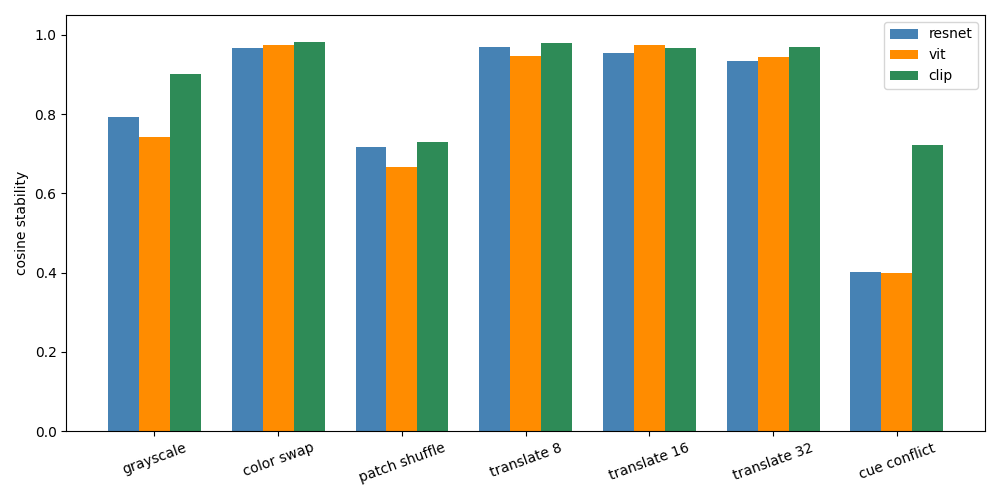
\includegraphics[width=\linewidth]{figures/task1_feature_stability.png}
  \end{minipage}\hfill
  \begin{minipage}{0.42\linewidth}
    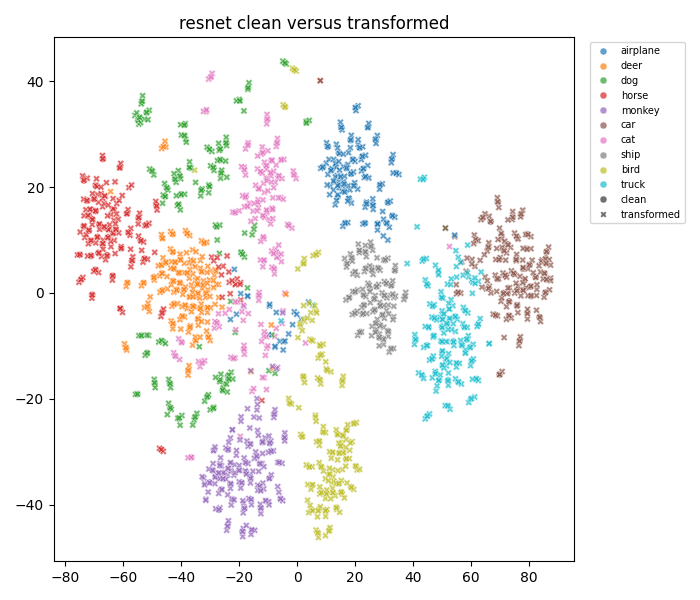
\includegraphics[width=\linewidth]{figures/task1_tsne_resnet.png}
  \end{minipage}
  \vspace{8pt}
  \caption{\textbf{CLIP's representation is the most stable of the three
  backbones under every intervention, including the two where its own
  accuracy drops most.} Left: cosine similarity between each backbone's
  clean and transformed features under every intervention. Right: a joint
  t-SNE projection of ResNet's clean (circle) and transformed (cross)
  features, colored by class, for a pool combining grayscale, patch shuffled,
  translated, and cue conflict images.}
  \label{fig:task1-stability}
\end{figure}

Figure~\ref{fig:task1-stability} shows prediction level and
representation level evidence mostly agree: patch shuffle and cue conflict
hurt accuracy most and also move features furthest from their clean
counterparts. Transformed points in the t-SNE projection still cluster
near their own class's clean cluster far more often than they cross into
another class's region, which is consistent with prediction accuracy
staying well above chance even under the largest feature shifts. CLIP is
the exception to the stability pattern. Its features stay the most stable
of the three under every intervention, which suggests the representation itself
drives these outcomes more than the classifier built on top of it. Patch
shuffling is also the one case that defies a simple locality story: CLIP
suffers the largest accuracy drop despite the convolution free ViT having
no locality prior at all. ViT's positional embeddings plausibly help it
reassociate shuffled patches, while CLIP, trained to match whole images
against whole captions, depends more on the overall composition staying
intact; that dependence points to CLIP's contrastive objective as the
likely source of its sensitivity to shuffled layout, a training signal ViT and
ResNet never received \citep{raghu2021vision}.

\section{Task 2: Unsupervised Domain Adaptation}
\label{sec:task2}

\subsection{Methodology}

A single ImageNet pretrained ResNet-18 is fine tuned on PACS's
three labeled source domains; Sketch supplies unlabeled images during
training and labeled images only at evaluation. Source-only cross entropy
is the baseline against three alignment methods. DAN adds a multi kernel
Maximum Mean Discrepancy penalty between source and target features before
the classifier head \citep{long2015learning}:
\begin{equation}
  \mathcal{L}_{\text{DAN}} = \mathcal{L}_{\text{cls}} + \lambda_{\text{MMD}}
  \left\lVert \mathbb{E}_s[\phi(F(x_s))] - \mathbb{E}_t[\phi(F(x_t))] \right\rVert^2_{\mathcal{H}}.
  \label{eq:mmd}
\end{equation}
MMD compares only a fixed, kernel based summary of the two feature
distributions, so a domain difference that kernel cannot see goes
unpenalized. DANN removes that dependence on a hand picked kernel
by learning the comparison itself: a domain discriminator sits behind a
gradient reversal layer, so backpropagation simultaneously minimizes
classification loss and maximizes domain confusion under a schedule that
ramps up reversal strength \citep{ganin2016domainadversarial}. That added
flexibility has a cost: it turns alignment into a minimax game between
discriminator and feature extractor instead of a single smooth penalty,
and minimax games are notoriously harder to stabilize. CDAN keeps the
adversarial discriminator but targets a different weakness: matching
the marginal feature distribution alone says nothing about whether
classes line up across domains. It conditions the discriminator on the
outer product of feature and predicted class distribution,
$g(x)=\mathrm{vec}(f\otimes p)$, so alignment follows class structure
instead of the marginal distribution alone \citep{long2018conditional}.
DANN and CDAN training also clips gradients to a norm of 5, L2
normalizes the features feeding the discriminator, and tunes the
learning rate per method, 3e-5 for DANN and the shared 1e-4 for CDAN. A
held out logistic regression probe distinguishing source from target
features gives a domain separability score, where 50 percent is chance.

\subsection{Results}

\begin{table}[H]
  \centering
  \small
  \begin{tabular}{lcccc}
    \toprule
    Method & Mean source acc. & Target (Sketch) acc. & Domain separability & Target $\Delta$ \\
    \midrule
    Source-only & 0.957 & 0.616 & 0.996 & -- \\
    DAN         & 0.942 & 0.643 & 0.894 & +0.026 \\
    DANN        & 0.955 & 0.715 & 0.999 & +0.099 \\
    CDAN        & 0.946 & 0.276 & 0.995 & -0.340 \\
    \bottomrule
  \end{tabular}
  \vspace{8pt}
  \caption{Task 2 method comparison. Only DAN's separability drop tracks
  its own target accuracy gain; DANN and CDAN's separability barely
  differs from source-only's despite their adversarial objective, so
  their numbers cannot be read as evidence about alignment quality.}
  \label{tab:task2-main}
\end{table}

Source-only already reaches 0.616 target accuracy from cross entropy,
well above chance, but leaves a near perfect domain
gap (separability 0.996) that is also uneven across classes: guitar
transfers almost perfectly since its outline barely changes across
styles, while giraffe and dog lose most of their accuracy, plausibly
leaning on color and texture cues Sketch lacks, a pattern invisible from
source domain validation alone. DAN narrows the domain gap to 0.894 and
lifts target accuracy to 0.643, but its per class numbers
(Table~\ref{tab:crosstask-dan})
show the gain is not uniform: most classes improve, some substantially,
while person collapses from 0.825 to 0.006, driven almost entirely by
person sketches classified as house (Appendix
Figure~\ref{fig:appendix-dan}).

DANN and CDAN both reach mean source accuracy in line with the other two
methods, 0.955 and 0.946, and DANN reaches 0.715 target accuracy, moving
past source-only's 0.616. CDAN's target accuracy stays low at 0.276. Its
confusion matrix (Appendix Figure~\ref{fig:appendix-cdan}) shows nearly
every Sketch image predicted as dog regardless of true class, while its
own source validation accuracy stays strong throughout. The failure is
specific to the target domain, since the shared backbone itself is
training normally.

The controlled sweep over DAN's MMD weight reinforces the picture: at
$\lambda_{\text{MMD}}=0.1$, $1.0$, and
$10.0$, mean source
accuracy is 0.9466, 0.9468, and 0.8834, target accuracy is 0.766, 0.661,
and 0.654, and domain separability is 0.986, 0.882, and 0.875. Separability
falls steadily as $\lambda_{\text{MMD}}$ rises, but target accuracy is
highest at the lowest weight tested, and mean source accuracy is
statistically indistinguishable between $\lambda_{\text{MMD}}=0.1$ and
$\lambda_{\text{MMD}}=1$ despite a ten point gap in target accuracy.

Lower domain separability tracks better target accuracy only for DAN;
DANN and CDAN's separability barely moves despite their adversarial
objective, so their target accuracy differences track how well each
classifier generalizes on its own instead of any working alignment
mechanism, and even DAN's own gain is uneven, since the same alignment
that helps most classes drives person's accuracy toward zero. CDAN's
class conditional discriminator is meant to prevent this kind of mixing,
yet its target domain collapse onto a single class still happens,
pointing to a degenerate solution specific to the unlabeled Sketch data
that a class balanced source domain evaluation would never show.

\section{Task 3: Domain Generalization}
\label{sec:task3}

\subsection{Methodology}

Task~3 reuses Task~2's exact source domain splits, backbone, and training
setup, with one restriction: no Sketch image, labeled or not, reaches
training, model selection, or hyperparameter choice; it appears only in
the final evaluation. Task~2's source-only checkpoint carries over
unchanged as the ERM baseline. DAN-DG applies the same MMD mechanism as DAN, but pairwise
across the three \emph{observed} source domains instead of between a
source and the target,
\begin{equation}
  \mathcal{L}_{\text{DAN-DG}} = \mathcal{L}_{\text{ERM}} + \frac{\lambda_{\text{DG}}}{3}
  \sum_{e<e'} \mathrm{MMD}^2\big(F(X_e), F(X_{e'})\big),
  \label{eq:dandg}
\end{equation}
testing whether invariance learned purely from the domains already
available transfers to one never seen. Aligning features is not the only
way to seek robustness: SAM instead asks whether the optimizer has
settled somewhere flat or sharp on the loss surface, independent of how
alike the domains look in feature space. It leaves the objective and the
set of domains untouched and changes only how the optimizer searches,
solving $\min_\theta
\max_{\lVert\epsilon\rVert_2\le\rho} \mathcal{L}_{\text{ERM}}(\theta+\epsilon)$
\citep{foret2021sharpnessaware} to seek parameters whose local loss
surface stays flat across a neighborhood of the optimum. A local
sharpness proxy, the increase in validation loss after one normalized
gradient ascent step, is measured for all three models on a fixed held
out batch.

\subsection{Results}

\begin{table}[H]
  \centering
  \small
  \begin{tabular}{lcccc}
    \toprule
    Method & Mean source acc. & Sketch acc. & Source separability & Sharpness \\
    \midrule
    ERM     & 0.957 & 0.616 & 0.860 & 0.321 \\
    DAN-DG  & 0.948 & 0.707 & 0.727 & 0.334 \\
    SAM     & 0.967 & 0.679 & 0.820 & 0.110 \\
    \bottomrule
  \end{tabular}
  \vspace{8pt}
  \caption{Task 3 method comparison. DAN-DG and SAM both beat the ERM
  baseline on Sketch through different mechanisms: DAN-DG lowers source
  separability, SAM lowers the sharpness proxy, and each method leaves the
  other's diagnostic largely unchanged.}
  \label{tab:task3-main}
\end{table}

Table~\ref{tab:task3-main} shows both proposed methods beating ERM
through visibly different mechanisms: DAN-DG lowers source domain
separability substantially and delivers the larger Sketch accuracy gain of
the two, while its sharpness proxy is no better than ERM's own; SAM moves
separability only slightly but drives sharpness down by nearly a factor
of three, yielding a smaller but still real Sketch accuracy gain. Mean
source accuracy is almost uninformative about this gap: all three methods
sit within a point of each other, yet SAM, highest on source accuracy, is
not highest on Sketch. Per class evidence (Table~\ref{tab:crosstask-dan})
shows DAN-DG's gain concentrated on elephant and giraffe at the cost of a
severe person collapse, strikingly similar to DAN's own Task~2 collapse
despite DAN-DG never touching Sketch during training. The collapse is
somewhat smaller for DAN-DG than for DAN, and that shared invariance
corresponds to DAN-DG's larger overall accuracy gain, but person
collapsing into elephant and giraffe instead of spreading evenly argues
that more invariance is not automatically better. Both methods also
trained smoothly, unlike Task~2's adversarial pair.

\begin{figure}[H]
  \centering
  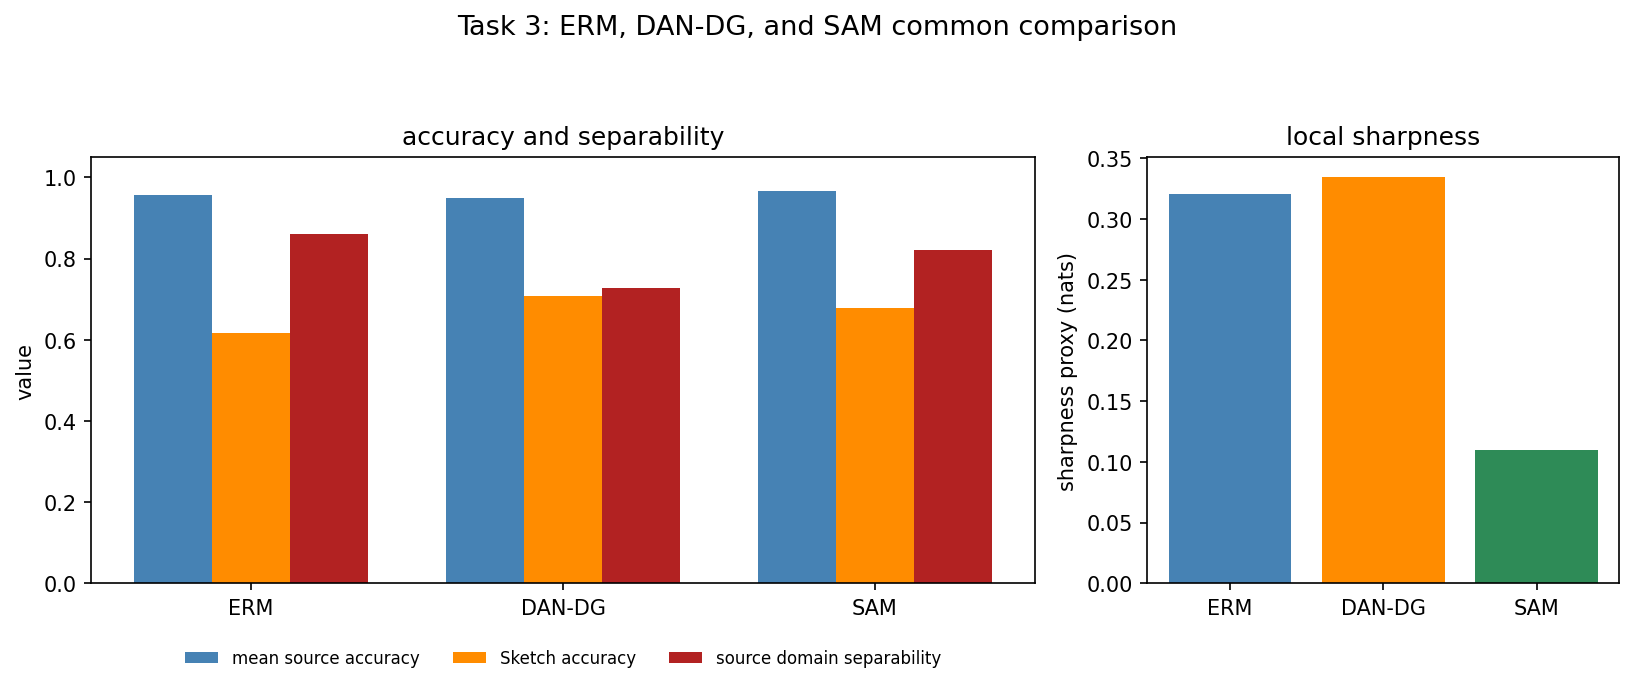
\includegraphics[width=0.86\linewidth]{figures/task3_method_comparison.png}
  \caption{\textbf{DAN-DG and SAM both beat ERM on Sketch, but through
  entirely different mechanisms.} Mean source accuracy, Sketch accuracy,
  source separability, and the local sharpness proxy for ERM, DAN-DG, and
  SAM. SAM's Sketch accuracy gain comes with a sharpness reduction of
  nearly a factor of three, while DAN-DG's larger gain comes with no
  sharpness improvement and a visibly
  lower separability instead.}
  \label{fig:task3-main}
\end{figure}

\begin{center}
\small
\begin{tabular}{lcc}
  \toprule
  Class & DAN (Task 2, target aware) & DAN-DG (Task 3, target free) \\
  \midrule
  dog      & +0.034 & +0.012 \\
  elephant & +0.161 & +0.381 \\
  giraffe  & +0.171 & +0.331 \\
  guitar   & -0.135 & -0.109 \\
  horse    & +0.038 & -0.023 \\
  house    & +0.138 & +0.025 \\
  person   & -0.819 & -0.631 \\
  \bottomrule
\end{tabular}
\captionof{table}{Per class Sketch accuracy change relative to the shared
ERM baseline, for Task 2's target aware DAN and Task 3's target free
DAN-DG. Both share the same large gains on elephant and giraffe and the
same person class collapse, despite only DAN having any access to Sketch
during training.}
\label{tab:crosstask-dan}
\end{center}

Sweeping SAM's perturbation radius $\rho$ over 0.01, 0.05, and 0.10 gives
mean source accuracy 0.959, 0.970, and 0.955, sharpness 0.234, 0.147, and
0.112, and Sketch accuracy 0.697, 0.748, and 0.715: sharpness falls
monotonically as $\rho$ rises, but Sketch accuracy peaks at the middle
value tested. $\rho=0.1$'s own training curve (Appendix
Figure~\ref{fig:appendix-sam}) shows why: mean validation macro-F1 sits at
or below chance for four epochs before recovering, an instability that
costs the accuracy gain the largest perturbation might otherwise have
earned.

Sketch accuracy alone reveals DAN-DG's alignment nearly erasing person;
source validation never shows it. SAM cuts sharpness sharply, yet that
ranking does not carry over to Sketch accuracy, since DAN-DG beats SAM
despite no sharpness edge: each method's own diagnostic supports only its
own mechanism, and neither explains the other's gain. Against Task~2's
target aware DAN, DAN-DG's target free alignment still generalized better,
though both share the
same person failure regardless of target access.

\section{Task 4: Open Set Recognition}
\label{sec:task4}

\subsection{Methodology}

A CIFAR appropriate ResNet-18 is trained from random initialization on all
ten CIFAR-10 classes (Vanilla), and again with RandAugment added (GCSC),
to ask whether stronger positive augmentation improves unknown rejection
alongside closed set accuracy. Four post hoc scores are then compared on
the frozen Vanilla model, each one turning its ordinary closed set logits
into a single unknownness score after training has already finished:
maximum softmax probability \citep{hendrycks2017baseline}, maximum logit
score \citep{vaze2022openset}, energy \citep{liu2020energybased}, and
Mahalanobis distance to the nearest class conditional Gaussian
\citep{lee2018simple}. PROSER \citep{zhou2021learning} takes the opposite
approach, changing what the network is trained to do. It fine tunes the Vanilla checkpoint
with five dummy classifiers under two objectives: a classifier placeholder
loss that pushes one dummy to be the second most confident response once
the true class is excluded, and a data placeholder loss that trains
manifold mixup interpolations between two known classes' features toward
those dummies. Together these let the network learn unknown like regions
without ever seeing real unknown data. Unknowns for every method come from two fixed
CIFAR-100 groups, near and far, that never influence training,
checkpoints, or thresholds; a threshold is calibrated once, on validation
data, to accept 95 percent of known images.

\subsection{Results}

\begin{table}[!htb]
  \centering
  \small
  \begin{tabular}{lccc}
    \toprule
    Score & Near AUROC & Far AUROC & All unknown AUROC \\
    \midrule
    MSP          & 0.819 & 0.902 & 0.861 \\
    MLS          & 0.796 & 0.905 & 0.851 \\
    Energy       & 0.796 & 0.906 & 0.851 \\
    Mahalanobis  & 0.807 & 0.920 & 0.864 \\
    \bottomrule
  \end{tabular}
  \\[6pt]
  \begin{tabular}{llcccc}
    \toprule
    Model & Score & CSA & Near AUROC & Far AUROC & All unknown AUROC \\
    \midrule
    Vanilla & MLS         & 0.947 & 0.796 & 0.905 & 0.851 \\
    GCSC    & MLS         & 0.951 & 0.816 & 0.910 & 0.863 \\
    PROSER  & MLS         & 0.942 & 0.789 & 0.876 & 0.832 \\
    PROSER  & Placeholder & 0.942 & 0.791 & 0.895 & 0.843 \\
    \bottomrule
  \end{tabular}
  \vspace{8pt}
  \caption{Top: post hoc novelty scores on the frozen Vanilla model; every
  score separates far unknowns far more easily than near unknowns. Bottom:
  Vanilla, GCSC, and PROSER compared on closed set accuracy (CSA) and
  near/far/all unknown AUROC.}
  \label{tab:task4-scores}
  \label{tab:task4-methods}
\end{table}

Mahalanobis distance is the best score overall, and on far unknowns
specifically. MSP is a close second, and MLS and Energy come next,
tracking the same raw logits within a point of each other. Mahalanobis's
edge is concentrated on far unknowns, suggesting feature space distance
captures something raw logits do not, while near unknowns stay hard for
every score alike precisely because they already resemble a known class.
At the calibrated threshold, near unknown acceptance stays high for every
score while far unknown acceptance is much lower.

GCSC's RandAugment approach improves closed set accuracy over
Vanilla and, under the same score, improves rejection on every axis too,
most on near unknowns, the harder group, plausibly because stronger
augmentation tightens each class's feature region where similarity would
otherwise let an unknown through. PROSER moves the opposite way:
known class accuracy sits slightly below Vanilla's, and MLS rejection is
worse on every axis. Its validation accuracy also oscillated across its
full run instead of converging smoothly the way Vanilla and GCSC's did
(Appendix Figure~\ref{fig:appendix-proser}). This is evidence that
manifold mixup interpolations are an imperfect stand in for real unknown
data, though the placeholder idea itself may still hold up with a better
interpolation scheme.

\begin{figure}[H]
  \centering
  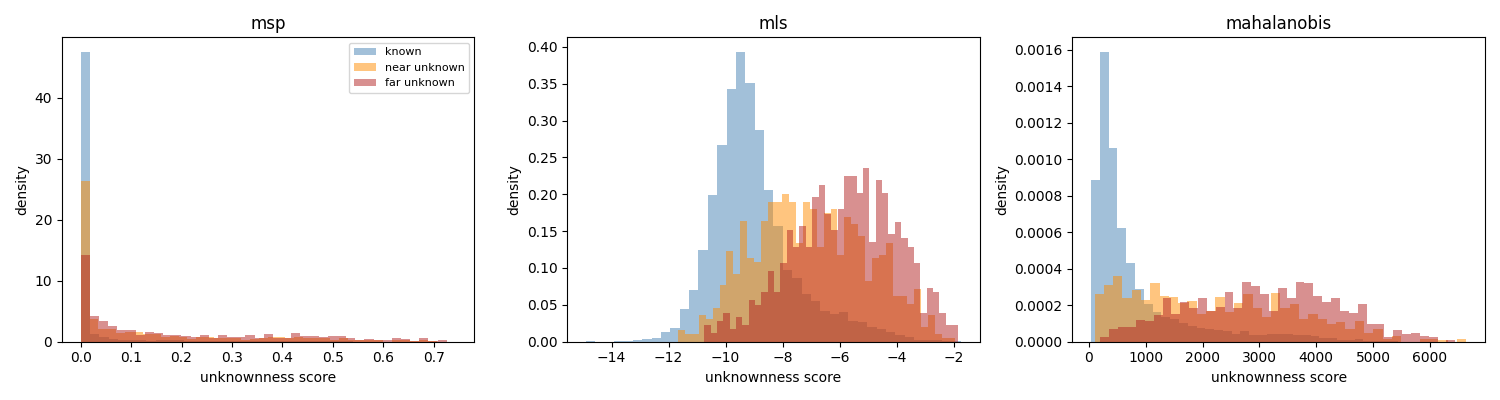
\includegraphics[width=\linewidth]{figures/task4_score_distributions.png}
  \caption{\textbf{Near unknown scores overlap heavily with known scores
  under every measure, while far unknown scores sit visibly apart.}
  Unknownness score distributions for known, near unknown, and far unknown
  images under MSP, MLS, and Mahalanobis.}
  \label{fig:task4-scores}
\end{figure}

The absorption pattern tracks semantic similarity closely. Among near
unknowns, pickup\_truck (94/100) and bus (82/100) are accepted almost as
often as a known vehicle, absorbed mostly into automobile and
truck, while motorcycle, least similar to any CIFAR-10 vehicle, is
accepted least of the eight (41/100); wolf, fox, leopard, and camel
absorb into cat, dog, deer, and horse. Far unknowns show the same
mechanism more weakly: wardrobe's boxy outline is often accepted as
truck or cat (62/100), and a handful of the most confident far unknown
failures have no obvious shared semantics at all, like a keyboard scored
as truck or a chair scored as cat:
\begin{center}
\small
\begin{tabular}{llccc}
  \toprule
  Group & Unknown class & Predicted known class & Score & Threshold \\
  \midrule
  Near & pickup\_truck & automobile & $-11.67$ & $-5.89$ \\
  Near & pickup\_truck & automobile & $-11.50$ & $-5.89$ \\
  Near & bus           & truck      & $-11.45$ & $-5.89$ \\
  Far  & chair         & cat        & $-10.75$ & $-5.89$ \\
  Far  & keyboard      & truck      & $-10.69$ & $-5.89$ \\
  Far  & bowl          & cat        & $-10.66$ & $-5.89$ \\
  \bottomrule
\end{tabular}
\captionof{table}{The most confidently accepted near and far unknown
failures under the maximum logit score, with the vanilla model's calibrated
threshold for reference.}
\label{tab:task4-failures}
\end{center}

That absence of shared semantics suggests the decision boundary follows
incidental texture and color correlations more than overall object
structure. GCSC's tightening of the feature space helps mainly on the
near unknown group, since far unknowns were already easy to reject
regardless of score or method; GCSC's plain augmentation remains the more
effective of the two closed set changes tried here for improving
rejection.

\section{Cross Task Discussion}
\label{sec:cross}

\paragraph{Visual cues and distribution shift.}
Task~1 finds patch shuffling and cue conflict hardest for every backbone,
both destroying global organization while leaving local structure intact.
PACS's Sketch domain removes an overlapping kind of evidence: texture and
color are gone, leaving something closer to a pure outline. Guitar and
house transfer best, because their outline alone nearly suffices; person,
giraffe, and dog transfer worst, likely because they lean on the color
and texture cues Task~1 showed these architectures partly depend on. This
resemblance is only suggestive. The datasets and architectures involved
differ too much to support a causal claim, but the pattern still points
toward a single shared vulnerability: ordinary supervised or contrastive
training leans on cues a real domain shift can remove entirely.

\paragraph{Invariance, discriminability, and target domain access.}
DAN and DAN-DG both make their domains harder to distinguish and both
improve mean target accuracy, but both do so at the cost of nearly
erasing person (Table~\ref{tab:crosstask-dan}). An overall feature
distribution penalty has no way to tell domain separating information
apart from class separating information, so this tradeoff is not
surprising. SAM tells a contrasting story: a real gain
with separability barely moved shows invariance is not the only route to
generalization. Each method's own diagnostic speaks only to its own
mechanism, and no single diagnostic here explains every method's gain.
DAN-DG's
target free alignment also outperformed DAN's target aware alignment, the
opposite of what valuable target access should produce. A single
benchmark cannot settle the general question, but target access is
clearly no substitute for a well behaved objective.

\paragraph{Recognition, rejection, and the overall picture.}
Closed set accuracy and unknown rejection moved together for GCSC but
apart for PROSER, echoing Tasks~1 and~2's lesson that an aggregate number
can hide the evidence that explains behavior. The near unknown
group was chosen for semantic closeness to known classes, and it is
consistently the harder case across every score and method. This is
exactly the case in which a confident classifier should sometimes
decline to answer.

\paragraph{Limitations.}
One limitation is that results depend on a single training run
rather than an average over multiple runs. Task~3 showed this matters:
SAM's own $\rho$ sweep at $\rho=0.1$ goes below chance for several epochs
before recovering (Appendix Figure~\ref{fig:appendix-sam}), an
instability large enough that a small gap between two methods, such as
DAN-DG's edge over SAM on Sketch, could just as easily come from random
training variation as from a real difference between the methods. A
second limitation is scope: each
paradigm here depends on one
benchmark and one backbone family, so the specific rankings between
methods, DAN-DG over SAM, or Mahalanobis over MSP, should be read as
evidence for this setting; extending them into a general claim would need
testing across multiple benchmarks.

\section{Conclusion}
\label{sec:conclusion}

Clean accuracy alone is not enough to trust a vision model, and these
four experiments show why in different ways. ResNet, ViT, and
CLIP reach near identical clean accuracy while relying on visibly
different evidence once color, shape, texture, and layout are
manipulated. DAN-DG and SAM reach a similar Sketch accuracy gain over the
shared ERM baseline for entirely different reasons, one by lowering
feature separability across source domains and the other by flattening
the loss surface, and neither method's own diagnostic explains the
other's success. DAN-DG even outperforms Task~2's target aware DAN on
Sketch despite never touching the target domain during training, so
target access is no substitute for a well behaved objective. Closed set
accuracy and unknown rejection moved together for GCSC but apart for
PROSER, so a classifier's performance on its own training distribution
says nothing about how well it rejects what falls outside it. Building a
robust vision system is less about maximizing a single number and more
about choosing what to preserve, what to treat as invariant, and when to
refuse to answer.

\clearpage
\bibliographystyle{plainnat}
\bibliography{references}

\clearpage
\appendix
\section{Appendix}
\label{sec:appendix}

DAN and CDAN's confusion matrices (Section~\ref{sec:task2}) are shown
here in full, along with training curves for SAM at $\rho=0.1$ and
PROSER (Sections~\ref{sec:task3} and~\ref{sec:task4}), both of which
show unstable training.

\subsection{DAN}

Figure~\ref{fig:appendix-dan} shows DAN's confusion matrix on Sketch as a
row percentage. Person sketches are predicted house 85 percent of the time, and
dog and elephant each lose roughly a third of their images to person the
same way; every other class stays mostly on its own diagonal.

\begin{figure}[H]
  \centering
  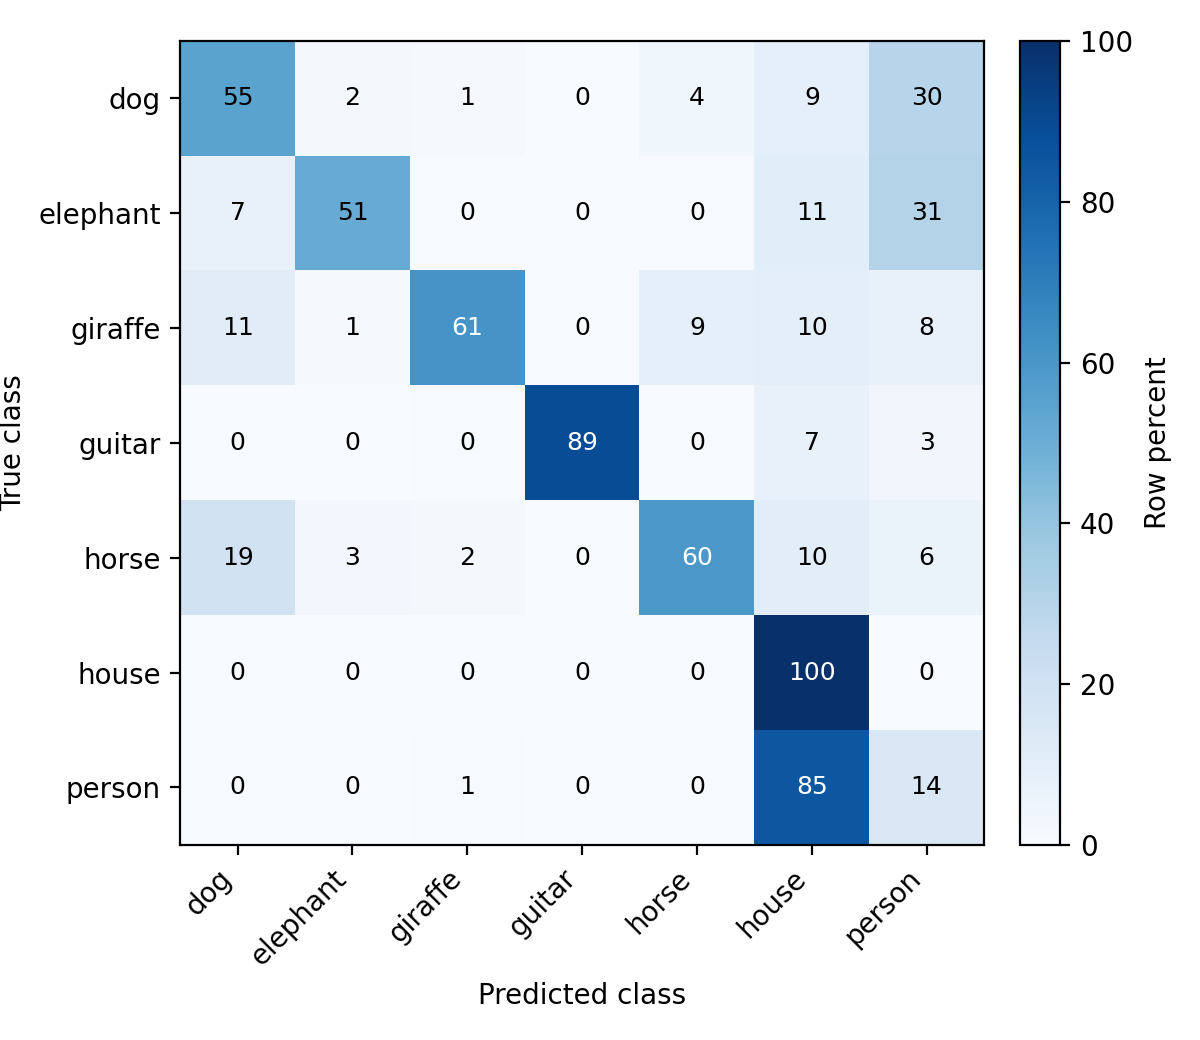
\includegraphics[width=0.6\linewidth]{figures/appendix_dan_confusion_matrix.png}
  \caption{DAN's confusion matrix on Sketch, as a percentage of each true
  class's images.}
  \label{fig:appendix-dan}
\end{figure}

\subsection{CDAN}

Figure~\ref{fig:appendix-cdan} shows CDAN's confusion matrix on Sketch as
a row percentage. Every class outside dog gets predicted dog most of the
time except house, which splits 40 percent dog and 60 percent correctly
as house; elephant and person are predicted dog for every single image.

\begin{figure}[H]
  \centering
  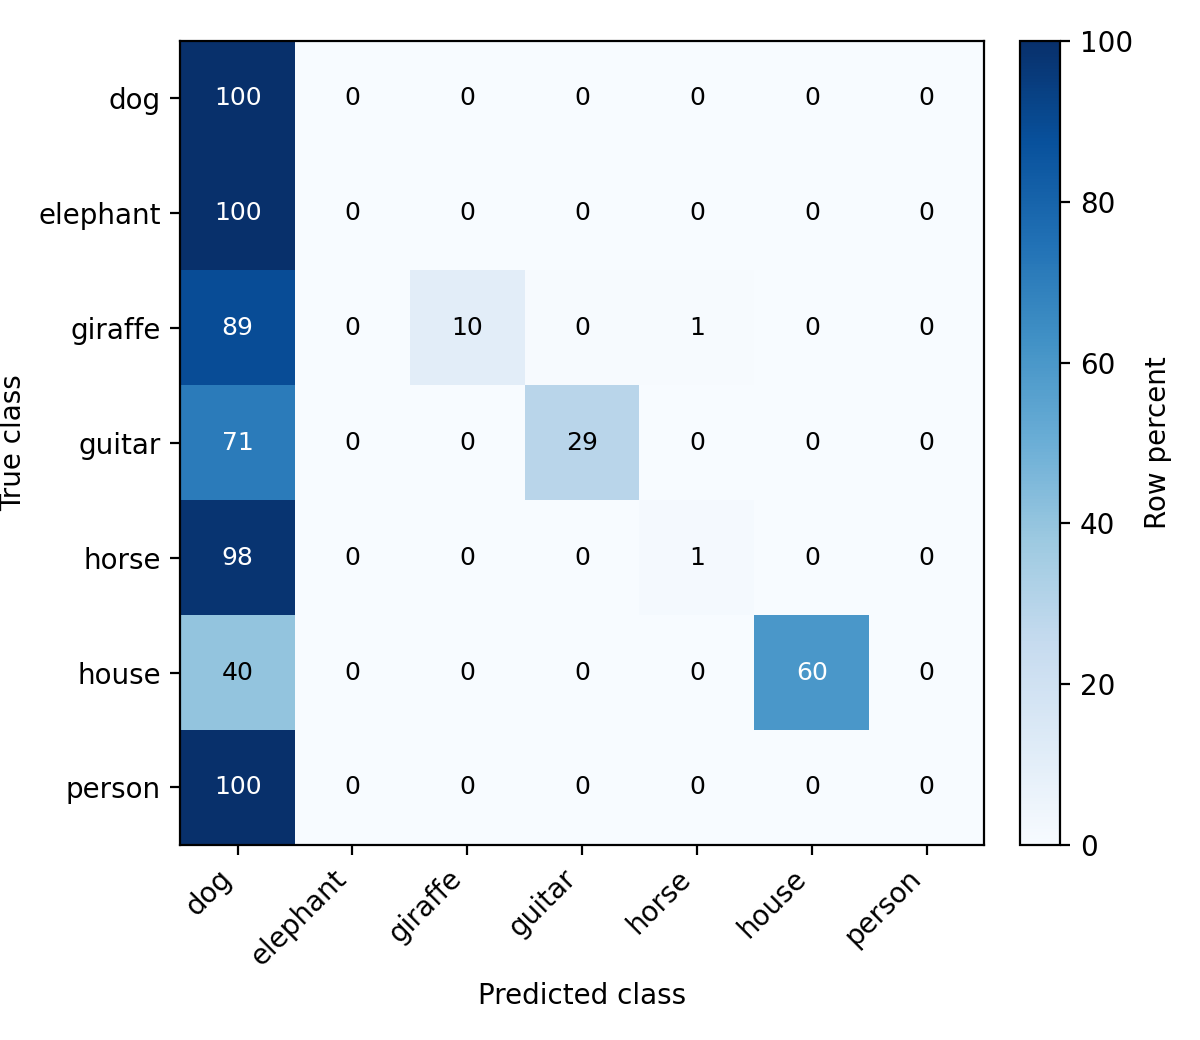
\includegraphics[width=0.6\linewidth]{figures/appendix_cdan_confusion_matrix.png}
  \caption{CDAN's confusion matrix on Sketch, as a percentage of each
  true class's images.}
  \label{fig:appendix-cdan}
\end{figure}

\subsection{SAM at \texorpdfstring{$\rho=0.1$}{rho=0.1}}

Figure~\ref{fig:appendix-sam} shows classification loss and mean source
validation macro F1 for the largest perturbation radius swept in
Section~\ref{sec:task3}. Validation macro F1 sits at or below chance for
the first four epochs before recovering, an instability that costs this
setting the accuracy edge a larger perturbation might otherwise earn.

\begin{figure}[H]
  \centering
  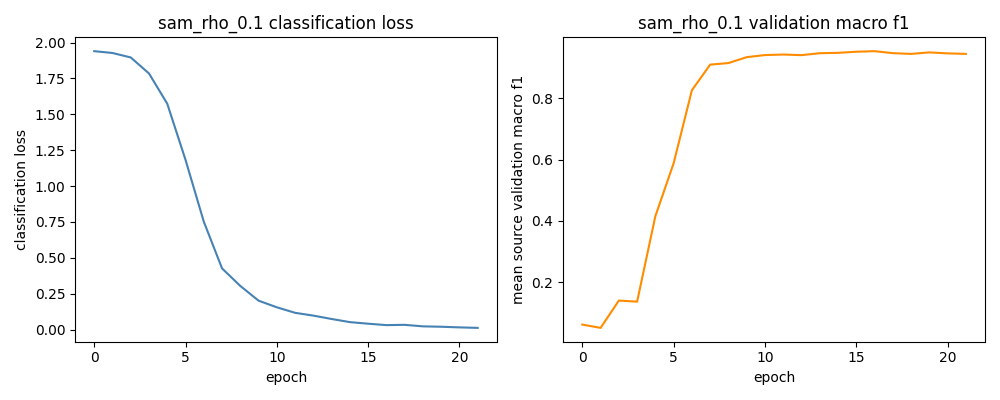
\includegraphics[width=0.88\linewidth]{figures/appendix_sam_rho0.1_training_curve.png}
  \caption{SAM's training curves at $\rho=0.1$.}
  \label{fig:appendix-sam}
\end{figure}

\subsection{PROSER}

Figure~\ref{fig:appendix-proser} shows training loss, validation
accuracy, and data placeholder loss across PROSER's full fifty epoch
fine tuning run. Validation accuracy oscillates for the entire run
instead of converging smoothly the way Vanilla and GCSC's own training
curves do.

\begin{figure}[H]
  \centering
  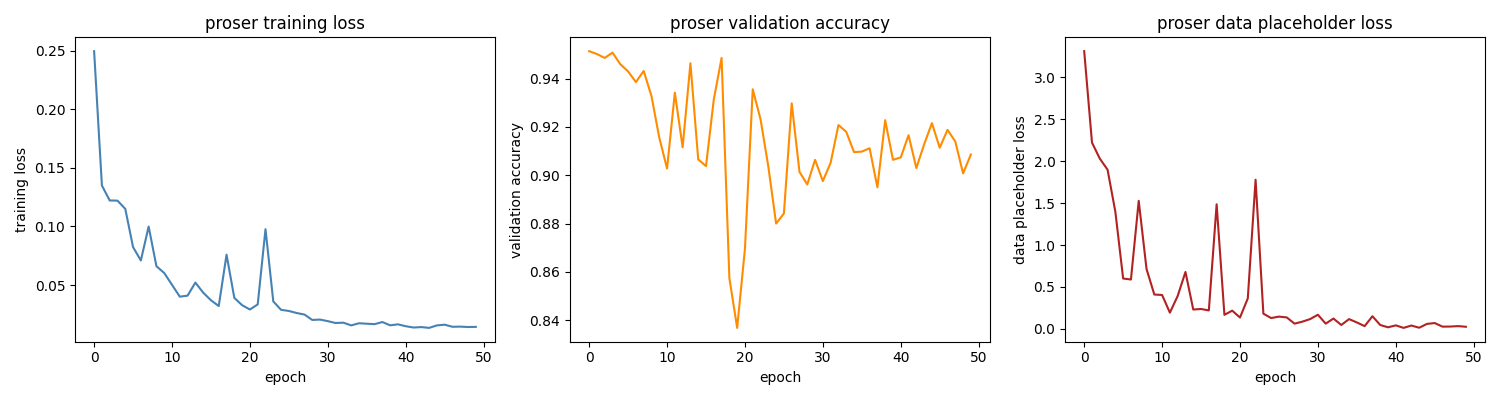
\includegraphics[width=0.95\linewidth]{figures/appendix_proser_training_curve.png}
  \caption{PROSER's training curves across its full fine tuning run.}
  \label{fig:appendix-proser}
\end{figure}

\end{document}
